\subsection{Few-shot updating from rapid mapping}\label{sec:res_fewshot}
Table~\ref{tab:fewshot} and Figure~\ref{fig:fewshot} summarise Experiment~2. Because updating changes only the offset, it leaves the ranking of cells unchanged, and HiPhyBoost keeps its advantage in discrimination over PC-GBM at every $k$ (median AUC 0.834--0.841 against 0.805--0.816). The differences between methods lie in the predicted landslide total and in its uncertainty.

\emph{Point accuracy.} After one mapped tile, recalibrated PC-GBM still mispredicts the landslide total in the unmapped area by a median factor of $2^{1.31}=2.5$, and the cell-level HiPhyBoost posterior by a factor of 2.2. The full HiPhyBoost quasi-posterior reduces this to a factor of 1.6 ($|\log_2 E/O|=0.68$), because a single tile no longer overrides the prior learned from eight past earthquakes. With five to ten tiles the error falls to a factor of about 1.4 (0.48--0.53), against 1.6 for recalibrated PC-GBM. All methods lose some accuracy at $k=40$, probably because the remaining unmapped area is then dominated by sparsely affected terrain, whose landslide density an offset fitted to the most affected tiles overstates.

\emph{Uncertainty.} The cell-level Bayesian posterior is far too confident. Its 90\% intervals contain the observed total in only 4--26\% of draws, because it treats the several thousand cells of a mapped tile as independent evidence. The measured dispersion of tile-level counts shows how wrong this is. Evaluated with each event's own fitted offset, $\phi$ ranges from 7 (Denali) to 193 (Cinchona). The values actually used in the update, the medians over the eight training events of each fold, are 47--68. A mapped tile therefore carries roughly one fiftieth of the information that the independence assumption gives it (Figure~\ref{fig:posterior}). The quasi-posterior raises coverage to 0.72--0.76 for $k\le 10$ and 0.70 at $k=20$. At the same time the interval for the remaining landslide total narrows from a factor of 59 after one tile to a factor of 6.5 after five and 3.7 after ten. Coverage stays below the nominal 90\% because a single dispersion factor cannot represent events as different as Denali and Cinchona, and it declines at $k=40$, when chosen tiles begin to share landslide clusters.

\emph{Selection.} Within the quasi-likelihood formulation the selection term has almost no effect (coverage 0.54 against 0.51 at $k=40$; otherwise identical). Once the likelihood is divided by $\phi$, the selection penalty is down-weighted by the same factor, and the bias it corrects is small compared with the dispersion. The selection term matters a great deal in the alternative Gaussian tile-random-effect formulation: there it raises coverage at $k=10$ from 0.20 to 0.74 and reduces the point error by about 40\%. That formulation, however, has a large point bias for the landslide total (factors of 2.5--4.4 after one to ten tiles). A Gaussian random effect cannot represent the real distribution of landslides over tiles, in which most tiles hold none and a few hold hundreds. We therefore recommend the quasi-posterior as the default form of component~(iii). The selection term costs nothing and protects against stronger targeting than our uniform-among-affected-tiles protocol simulates.

\begin{table*}[t]\centering\small
\caption{Few-shot updating from $k$ rapidly mapped $3\times3$~km tiles (Experiment~2; identical tile draws for all methods, 30 repetitions per event and $k$). $|\log_2 E/O|$: absolute log$_2$ ratio of predicted to observed landslide cells in the unmapped area (median over events of per-event medians; 1 = a factor of two). Coverage: share of draws in which the 90\% predictive interval contained the observed total (mean over events; nominal 0.90). Width: ratio of the upper to the lower interval bound (median).}\label{tab:fewshot}
\resizebox{\textwidth}{!}{\begin{tabular}{lrrrrrrrrrr}\toprule
 & \multicolumn{4}{c}{$|\log_2 E/O|$} & \multicolumn{4}{c}{90\% coverage} & \multicolumn{2}{c}{Width}\\\cmidrule(lr){2-5}\cmidrule(lr){6-9}\cmidrule(lr){10-11}
Method & $k$=1 & 5 & 10 & 40 & 1 & 5 & 10 & 40 & $k$=1 & 10\\\midrule
PC-GBM, intercept recalibration & 1.31 & 0.64 & 0.71 & 0.64 & -- & -- & -- & -- & -- & --\\
PC-GBM, Platt recalibration & 1.37 & 0.69 & 0.68 & 0.67 & -- & -- & -- & -- & -- & --\\
HiPhyBoost, ML offset & 1.17 & 0.62 & 0.52 & 0.60 & -- & -- & -- & -- & -- & --\\
HiPhyBoost, cell-level Bayes & 1.14 & 0.64 & 0.52 & 0.60 & 0.26 & 0.19 & 0.16 & 0.04 & 2.3 & 1.2\\
\quad + selection term & 1.14 & 0.61 & 0.52 & 0.59 & 0.26 & 0.19 & 0.17 & 0.04 & 2.3 & 1.2\\
HiPhyBoost, tile random effect & 2.57 & 2.26 & 2.27 & 2.38 & 0.79 & 0.44 & 0.20 & 0.00 & 70 & 6.0\\
\quad + selection term & 2.15 & 1.35 & 1.37 & 1.47 & 0.82 & 0.85 & 0.74 & 0.19 & 114 & 9.2\\
HiPhyBoost, quasi-Bayes & 0.66 & 0.52 & 0.48 & 0.58 & 0.73 & 0.74 & 0.72 & 0.51 & 58 & 3.7\\
\quad + selection term (full HiPhyBoost) & 0.68 & 0.53 & 0.48 & 0.58 & 0.73 & 0.74 & 0.72 & 0.54 & 59 & 3.7\\
\bottomrule\end{tabular}}\end{table*}


\begin{figure*}[t]\centering
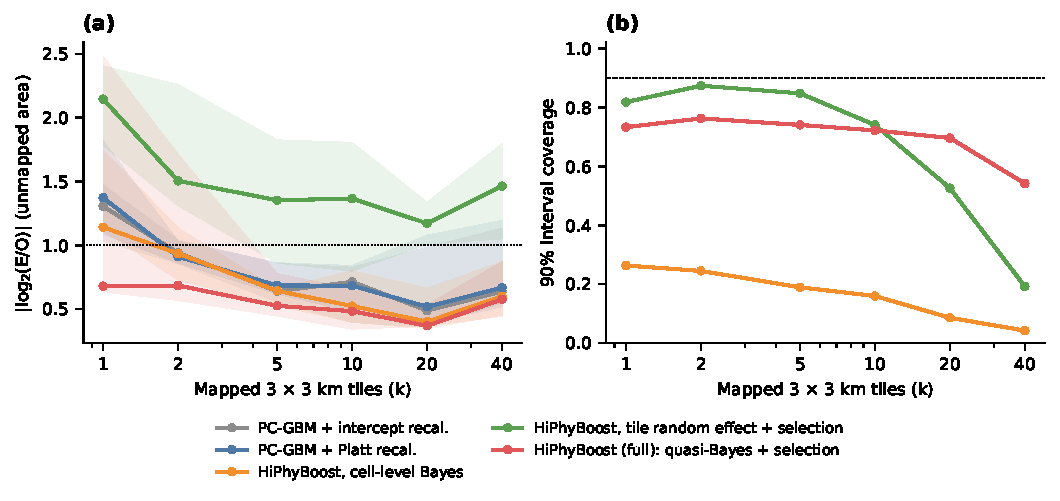
\includegraphics[width=\textwidth]{fig5_fewshot.pdf}
\caption{Few-shot updating from $k$ rapidly mapped $3\times3$~km tiles, evaluated on the unmapped part of each held-out event. (a) Absolute $\log_2$ ratio of predicted to observed landslide cells (1 = a factor of two); (b) coverage of the 90\% predictive interval of the landslide total (dashed: nominal). Lines: median (a) or mean (b) over events; shading: interquartile range over events. At $k=40$, Niigata-Chuetsu is excluded because it has fewer than 80 tiles.}\label{fig:fewshot}
\end{figure*}

\begin{figure*}[t]\centering
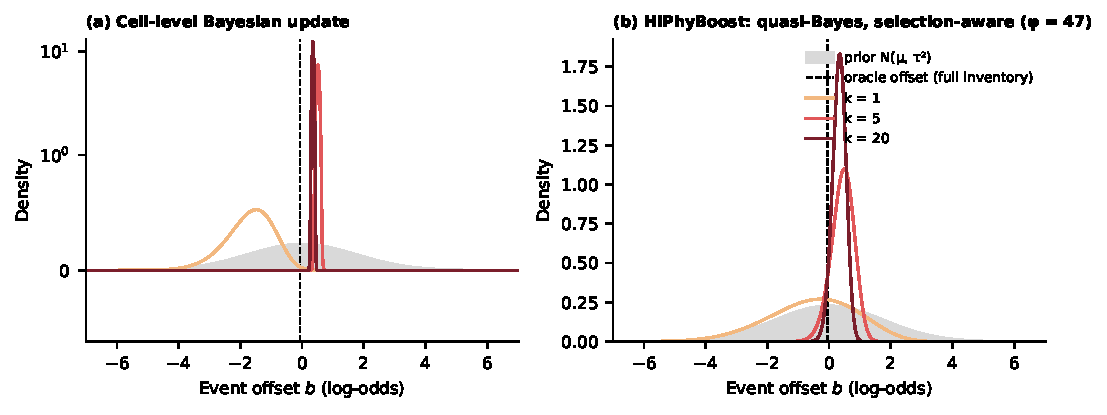
\includegraphics[width=\textwidth]{fig9_posterior_kaikoura.pdf}
\caption{Posterior of the Kaik\={o}ura event offset after mapping $k=1$, 5 and 20 randomly chosen landslide-bearing tiles, using HiPhyBoost scores transferred from the eight other earthquakes. (a) A cell-level Bayesian update (note the logarithmic density axis) concentrates on a wrong value after a few tiles. (b) The HiPhyBoost quasi-posterior with dispersion factor $\phi$ narrows gradually and stays consistent with the offset implied by the complete inventory (dashed).}\label{fig:posterior}
\end{figure*}
